\documentclass{beamer}

\usepackage{graphicx,color,transparent,amsmath,url}

\useoutertheme{infolines}
\usetheme{default}
\setbeamertemplate{navigation symbols}{}

\title[Odometry and Path Following]{%
  \normalsize
  Halmstad University course DT8007 (2013)\\
  Design of Embedded Intelligent Systems\\[2\baselineskip]
  \Large
  \textbf{Odometry and Path Following}\\
  for Differential-Drive Robots}
\author{Roland Philippsen}
\institute{Halmstad University}

\begin{document}

\begin{frame}[plain]
  \titlepage
  \vfill
  \begin{minipage}{\columnwidth}
    \centering
    \begin{minipage}{0.15\columnwidth}
      
\includegraphics[width=\columnwidth]{by-sa.pdf}
    \end{minipage}
    \hspace{1mm}
    \begin{minipage}{0.7\columnwidth}
      \tiny
      Except where otherwise noted,
      this work is licensed under a Creative Commons Attribution-ShareAlike 3.0 Unported License.
      \url{http://creativecommons.org/licenses/by-sa/3.0/}
    \end{minipage}
  \end{minipage}
\end{frame}

\begin{frame}<beamer>
  \frametitle{Outline}
  \tableofcontents
\end{frame}


\section{Foundations of Motion Control}


\begin{frame}{Wheel Control}
  
  \begin{minipage}{0.3\columnwidth}
    \textbf{CPU}\\
    $\downarrow$ motor command $u$\\
    \textbf{board}\\
    $\downarrow$ motor tension [V]\\
    \textbf{motor}\\
    $\downarrow$ $\dot\beta$ [rad/s]\\
    \textbf{gear} $N_\text{w}:N_\text{m}$\\
    $\downarrow$ $\dot\beta N_\text{w} = \pm \dot\alpha N_\text{m}$\\
    \textbf{wheel} radius $R$ [m]\\
    $\downarrow v = R \dot\alpha$\\
    \textbf{velocity} [m/s]
  \end{minipage}
  \hfill
  \begin{minipage}{0.65\columnwidth}    
    \def\svgwidth{\columnwidth}
    \input{wheel-control.pdf_tex}
  \end{minipage}
  
  \vfill
  
  \begin{itemize}
  \item
    left and right wheels: subscripts l and r
  \item
    motor command (1 byte) $u_\text{l,r} \leftrightarrow \dot\alpha_\text{l,r}$
  \item
    encoder counter (4 bytes) $e_\text{l,r} \leftrightarrow \alpha_\text{l,r} = \int \dot\alpha_\text{l,r} dt \approx \sum\Delta\alpha_\text{l,r}$
  \end{itemize}
  
\end{frame}


\begin{frame}{Velocity and Acceleration Limits}
  
  \textbf{Avoid jumps in velocity commands!}
  
  \vfill
  
  \begin{minipage}{0.4\columnwidth}    
    \begin{align*}
      \Delta p_\text{min}
      &=
      \frac{1}{2} v \cdot t_\text{min} = \frac{v^2}{2 \cdot a_\text{max}}
      \\
      \Delta p
      &=
      p_\text{goal} - p
    \end{align*}
  \end{minipage}
  \hfill
  \begin{minipage}{0.4\columnwidth}
    \def\svgwidth{\columnwidth}
    \input{trapezoidal-velocity.pdf_tex}
  \end{minipage}
  
  \vfill
  
  \begin{itemize}
    
  \item
    desired velocity $v_\text{des}$ also depends on timestep $\Delta t$
    
  \item
    for $v \geq 0$
    \[
    \begin{cases}
      \Delta p_\text{min} < \Delta p
      &\rightarrow
      \begin{cases}
        v < v_\text{max} - a_\text{max} \cdot \Delta t
        &\rightarrow
        v_\text{des} = v + a_\text{max} \cdot \Delta t
        \\
        \text{else}
        &\rightarrow
        v_\text{des} = v_\text{max}
      \end{cases}
      \\
      \text{else}
      &\rightarrow
      v_\text{des} = v - a_\text{max} \cdot \Delta t
    \end{cases}
    \]
    
  \item
    for negative $v$ you need to flip some signs\ldots
    
  \end{itemize}
  
\end{frame}


\begin{frame}{Velocity and Acceleration Limits}
  
  \textbf{Too simplistic!} $\rightarrow$ add lookahead, ``dead band,'' PD control, \ldots

  \includegraphics[width=\textwidth]{simplistic-trapezoidal-profiles.pdf}
  
\end{frame}

\section{Kinematics and Odometry}


\begin{frame}{Differential-Drive Kinematics}
  
  \begin{minipage}{0.5\columnwidth}
    In \textbf{local} frame:
    \vspace{-0.5\baselineskip}
    \begin{align*}
      \Delta\theta
      &=
      \omega \Delta t
      \\
      \Delta x
      &=
      \begin{cases}
        \text{arc} \rightarrow
        &
        S \sin \Delta \theta
        \\
        \text{else}
        &
        L \cos (\Delta \theta / 2)
      \end{cases}
      \\
      \Delta y
      &=
      \begin{cases}
        \text{arc} \rightarrow
        &
        S (1 - \cos \Delta \theta)
        \\
        \text{else}
        &
        L \sin (\Delta \theta / 2)
      \end{cases}
      \\
      \text{where}
      \\
      v_\text{l,r}
      &=
      \dot\alpha_\text{l,r} \cdot R_\text{l,r}
      \\
      v
      &=
      (v_\text{l} + v_\text{r}) / 2
      \\
      \omega
      &=
      (v_\text{r} - v_\text{l}) / B
      \\
      L
      &=
      v \Delta t
      \\
      S
      &=
      v / \omega
    \end{align*}
    
  \end{minipage}%
  \begin{minipage}{0.3\columnwidth}
    
    \def\svgwidth{1.4\columnwidth}
    \input{kinematics.pdf_tex}

    In \textbf{global} frame:
    \vspace{-0.5\baselineskip}
    \begin{align*}
      x^+
      &=
      x^- + \Delta x \cos \theta - \Delta y \sin \theta
      \\
      y^+
      &=
      y^- + \Delta y \cos \theta + \Delta x \sin \theta
      \\
      \theta^+
      &=
      \theta^- + \Delta \theta
    \end{align*}
    
  \end{minipage}
  
\end{frame}


\begin{frame}{Rotate-Translate-Rotate Control (RTR)}
  
  \def\svgwidth{\columnwidth}
  \input{rtr.pdf_tex}
  
\end{frame}


\begin{frame}{Odometry Calibration}
  
  \centering
  \fbox{\parbox{0.8\columnwidth}{
  \begin{align*}
    \Delta \theta
    &=
    \frac{\Delta p_\text{r} - \Delta p_\text{l}}{B}
    &
    \Delta p_\text{l,r}
    &=
    R_\text{l,r} \Delta \alpha_\text{l,r}
    \\
    L
    &=
    \frac{\Delta p_\text{l} + \Delta p_\text{r}}{2}
    &
    \alpha_\text{l,r}
    &=
    \frac{2 \pi N_\text{w}}{N_\text{e} N_\text{m}} e_\text{l,r}
  \end{align*}}}
  
  \vfill
  
  \begin{minipage}[t]{0.45\columnwidth}
    \textbf{1.\ determine $\bar{R} = (R_\text{l}+R_\text{r})/2$}
    \begin{align*}
      L
      &=
      \Delta\bar{p} = \bar{R} \Delta\bar{\alpha}
      \\
      &=
      (2 \pi N_\text{w} \bar{R} \Delta{\bar{e}}) / (N_\text{e} N_\text{m})
      \\
      \bar{R}
      &=
      \frac{N_\text{e} N_\text{m} L}{2\pi N_\text{w} \Delta\bar{e}}
    \end{align*}
    unknown $N$? $\rightarrow$ use $L = R^\ast\Delta{\bar{e}}$
  \end{minipage}
  \hfill
  \begin{minipage}[t]{0.45\columnwidth}
    \textbf{2.\ determine $B$}
    \begin{align*}
      B
      &=
      (\Delta p_\text{r} - \Delta p_\text{l}) / \Delta\theta
      \\
      &=
      \bar{R}(\Delta\alpha_\text{r} - \Delta\alpha_\text{l}) / \Delta\theta
      \\
      &=
      \frac{2\pi\bar{R}N_\text{w}}{N_\text{e}N_\text{m} \Delta\theta} (\Delta e_\text{r} - \Delta e_\text{l})
    \end{align*}
    try $\Delta\theta = 2k\pi$ with $k\in\mathbb{N}$
  \end{minipage}
    
\end{frame}


\begin{frame}{Odometry Calibration}
  
  \textbf{Beware of $R_\text{l} \ne R_\text{r}$}
  
  \vfill
  
  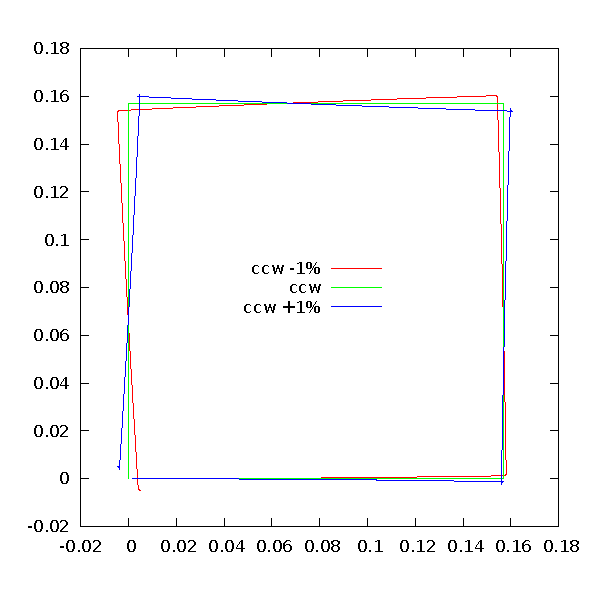
\includegraphics[width=0.5\columnwidth]{odom-ccw.pdf}%
  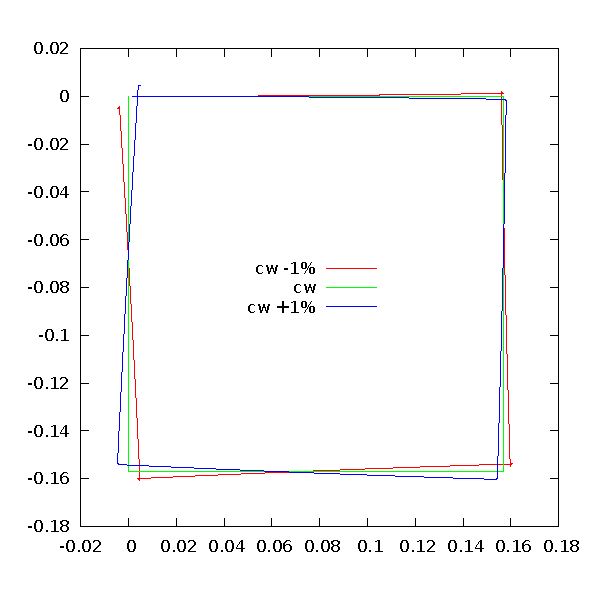
\includegraphics[width=0.5\columnwidth]{odom-cw.pdf}
  
  \vfill
  For more information, visit\\
  \url{http://www-personal.umich.edu/~johannb/umbmark.htm}
  
\end{frame}  


\section{Path Following}


\begin{frame}{Pose Feedback Control}
  
  \begin{minipage}{0.45\columnwidth}
    \def\svgwidth{\columnwidth}
    \input{ptctrl.pdf_tex}
  \end{minipage}
  \begin{minipage}{0.5\columnwidth}
    polar error:
    \vspace{-\baselineskip}
    \begin{align*}
      \Delta x
      &=
      x_\text{goal} - x
      \\
      \Delta y
      &=
      y_\text{goal} - y
      \\
      \epsilon
      &=
      \text{atan2}(\Delta y, \Delta x)
      \\
      \rho
      &=
      \sqrt{\Delta x^2 + \Delta y^2}
      \\
      \gamma
      &=
      \epsilon - \theta
      \\
      \delta
      &=
      \theta_\text{goal} - \gamma - \theta
      \\
      \text{with}
      &\quad
      \gamma, \delta \in (-\pi, \pi)
    \end{align*}
  \end{minipage}
  
  \vfill
  \begin{itemize}
  \item
    desired speed:
    $v = k_\rho \rho,\quad \omega = k_\gamma \gamma + k_\delta \delta$\\
    \emph{but beware of velocity limits!}
  \item
    stability:
    $k_\rho > 0,\quad k_\delta < 0,\quad k_\gamma + \frac{5}{3}k_\delta - \frac{2}{\pi}k_\rho > 0$
  \end{itemize}
  
  \hfill\tiny\emph{[Siegwart and Nourbakhsh. Introduction to Autonomous Mobile Robots. MIT Press, ISBN 0-262-19502-X.]}
\end{frame}


\begin{frame}{Uniform Cubic B-Spline}
  
  \begin{align*}
    q_i(\tau) &= \sum_{k=-1}^{2}b_{k}(\tau)p_{i+k}
    &
    \text{where}
    \begin{cases}
      b_{-1}     &= (-\tau^3 + 3\tau^2 - 3\tau + 1) / 6 \\
      b_0       &= (3\tau^3 - 6\tau^2 + 4) / 6 \\
      b_1       &= (-3\tau^3 + 3\tau^2 + 3\tau + 1) / 6 \\
      b_2       &= \tau^3 / 6 \\
      \tau      &\in [0,1]
    \end{cases}
  \end{align*}
  
  \begin{minipage}{0.25\columnwidth}
    \centering
    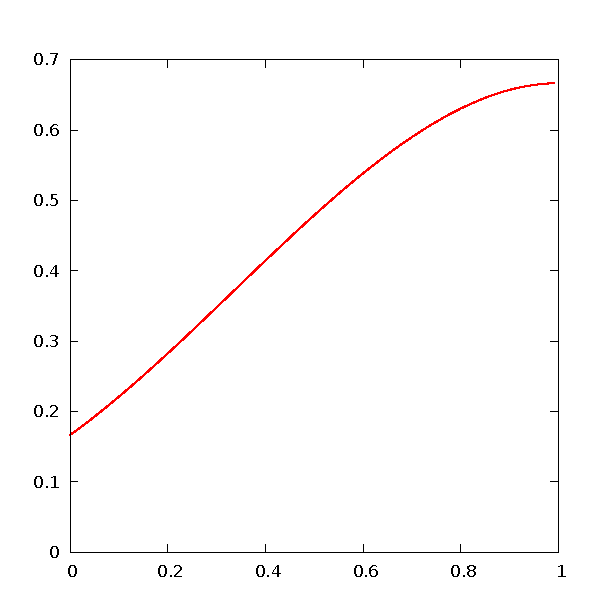
\includegraphics[width=\columnwidth]{b2.pdf}\\
    $b_2$
  \end{minipage}%
  \begin{minipage}{0.25\columnwidth}
    \centering
    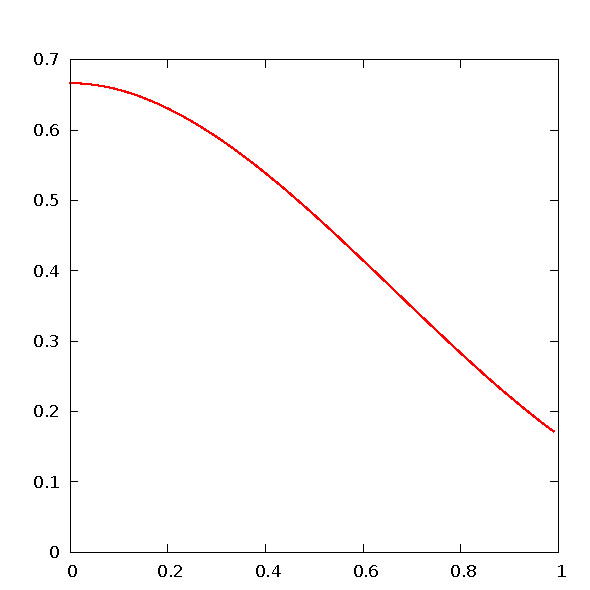
\includegraphics[width=\columnwidth]{b1.pdf}\\
    $b_1$
  \end{minipage}%
  \begin{minipage}{0.25\columnwidth}
    \centering
    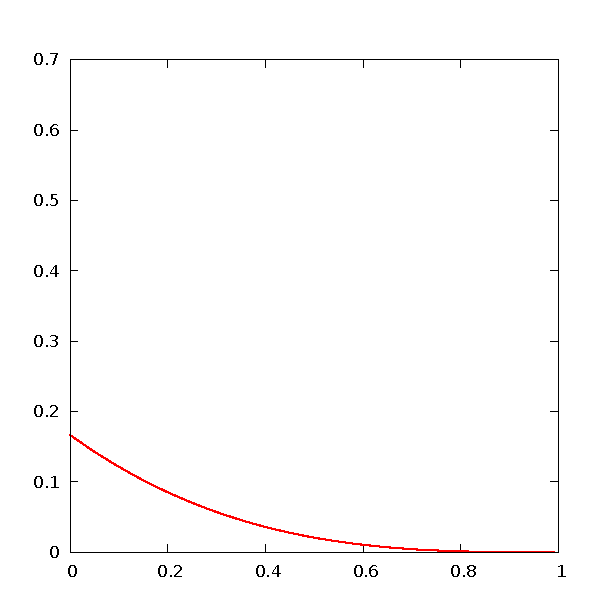
\includegraphics[width=\columnwidth]{b0.pdf}\\
    $b_0$
  \end{minipage}%
  \begin{minipage}{0.25\columnwidth}
    \centering
    \includegraphics[width=\columnwidth]{b-1.pdf}\\
    $b_{-1}$
  \end{minipage}
  
\end{frame}


\begin{frame}{Following (Spline) Paths}
  
  \centering
  %%  \includegraphics[width=0.5\columnwidth]{spline-ulf-1.pdf}%
  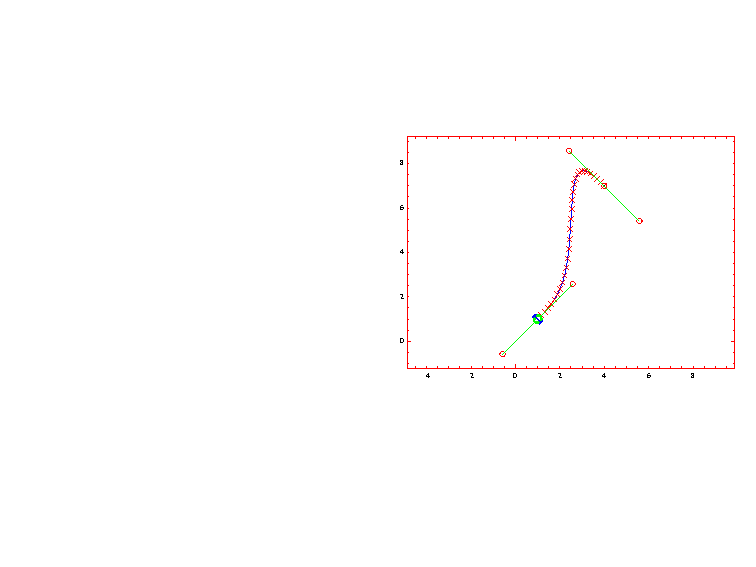
\includegraphics[width=0.5\columnwidth]{spline-ulf-2.pdf}
  
  \begin{minipage}[t]{0.45\columnwidth}
    Basic idea:
    \begin{itemize}
    \item
      Compute a $p_\text{goal}$ that moves along the spline with a nice velocity profile.
    \item
      Use feedback controller to follow $p_\text{goal}$
    \end{itemize}
  \end{minipage}
  \hfill
  \begin{minipage}[t]{0.45\columnwidth}
    Ingredients:
    \begin{itemize}
    \item
      Choice of control points?
    \item
      How to compute $\theta_\text{goal}$?
    \item
      How to advance $\tau$?
    \end{itemize}
  \end{minipage}
  
\end{frame}


\begin{frame}{Integration with Localization}
  \centering
  (If time allows\ldots)
\end{frame}


\section{Take Home Message}

\begin{frame}{Take Home Message}

\begin{itemize}

\item
  Underlying Control Capabilities
  \begin{itemize}
  \item
    wheel speed $\dot\alpha\leftrightarrow$ motor command $u$
  \item
    acceleration \& speed limts $\leftrightarrow$ trapezoidal velocity
  \item
    RTR $v_\text{l}=\pm v_\text{r}$ good for odometry calibration
  \end{itemize}

\item
  Dealing with Differential-Drive Kinematics
  \begin{itemize}
    \item
      $\{\dot\alpha_\text{l},\dot\alpha_\text{r}\} \leftrightarrow \{v,\omega\}$ with parameters $\{R_\text{l}, R_\text{r}, B\}$
    \item
      odometry: $\{\Delta e_\text{l}, \Delta e_\text{r}\} \rightarrow \{v,\omega\} \rightarrow \{\Delta x, \Delta y, \Delta \theta\}$
    \item
      pose control: $\{\rho, \gamma, \delta\} \rightarrow \{v,\omega\}$ good for short distances
  \end{itemize}

\item
  Path Following
  \begin{itemize}
  \item
    feedback control to a ``carrot'' (goal pose)
  \item
    splines: smooth paths, but careful about velocity profile
  \item
    avoiding control jumps due to localization jumps
  \end{itemize}
\end{itemize}

\end{frame}


\end{document}

